\documentclass{article}

\usepackage{amsmath,amssymb}
\usepackage{fullpage}
\usepackage{enumerate}
\usepackage{hyperref}
\usepackage{graphicx}
\graphicspath{{../logos/}}


\begin{document}

\setlength{\tabcolsep}{6pt}
\begin{center} \begin{tabular}{cccc}
	
\includegraphics[height=56pt]{SAMF_logo.jpg} &
	
\includegraphics[height=56pt]{SAICA_logo.jpg} &
	
\includegraphics[height=56pt]{OM_Logo_Stacked_Vignette_on_White_RGB.jpg} &
	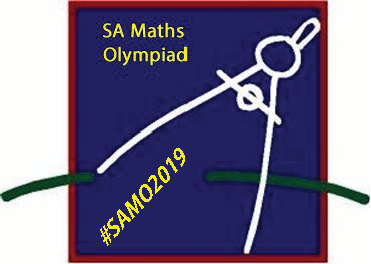
\includegraphics[height=56pt]{SAMO2019.png}
\end{tabular} \end{center}


\bigskip


\begin{center}
	\textbf{\Large Senior January Monthly Problem Set Solutions}
\end{center}

\begin{enumerate}

\medskip
\item % PAMO Shortlist 2019
{\itshape On the board, we write the integers $1, 2, 3, \dots, 2019$.
At each minute, we pick two numbers on the board $a$ and $b$, erase them, and write down the number $s(a + b)$ instead where $s(n)$ denotes the sum of the digits of the integer $n$.
Let $N$ be the last number remaining on the board.
\begin{enumerate}
	\item Is it possible that $N = 19$?
	\item Is it possible that $N = 15$?
\end{enumerate}}

Since $10^{n} \equiv 1 \pmod 3$ for all non-negative integers $n$, we have that $s(n) \equiv n \pmod 3$ and so replacing $a$ and $b$ with $s(a+b)$ does not change the sum of the numbers on the board in mod 3. 
Now $1 + 2 +... + 2019 = \frac{(2019)(2020)}{2} \equiv 0 \pmod 3$ but $19 \not\equiv 0 \pmod 3$ so we cannot have $N=19$ as the last number on the board. 

We now show that we can in fact get to $15$. 

For each $k \neq \{1010, 906\}$, replace the numbers $k$ and $2020-k$ with $s(k + 2020-k) = s(2020)$ = $4$. So remaining on the board now is $906, 1114, 1010$ and $1008$ $4$s. Now taking the $4$s in pairs and applying the procedure gives $504$ $8$s, taking these in pairs gives $252$ $7$s, and taking these $7$s in pairs gives $126$ $5$s and again taking these $5$s as pairs gives $63$ $1$s. So we have left $906, 1114, 1010$ and $63$ $1$s. Now apply the procedure in $1114$ and $1010$ to get $s(2125)=9$ and remain with $9, 906$ and $63$ $1$s. Now from the $63$ $1$s, we can make $7$ $9$s by taking $1$s and applying the procedure until we get to a $7$ then we stop and take a $1$ that has not been used. We then have $8$ $9$s and $906$ left on the board. Since $s(9 + 9) = s(18) = 9$, we can apply this procedure to the $9$s until just one $9$ remains. Finally, we combine this $9$ with the $906$ to get $s(906 + 9) = s(915) = 15$.

Remark: {\itshape The steps used to get to 15 are not unique.}

\medskip
\item % Baltic Way 2009 Problem 8
{\itshape For which positive integers $n$ is it possible to divide the set of numbers $\{n, n+1, n+2, \dotsc, n+8\}$ into two disjoint sets $A$ and $B$ such that the product of the numbers in $A$ is equal to the product of the numbers in $B$?}

Let $S = \{n, n+1, \dotsc, n+8\}$.
Without loss of generality let $A$ have more elements than $B$; since we have $9$ elements in total, it is impossible for them to have the same number of elements, and $\#A +\#B = 9$ gives that $A$ has at least $5$ elements and $B$ has at least $4$ elements.
The $5$ smallest elements of $S$ are $n$, $n+1$, $n+2$, $n+3$, and $n+4$, while the $4$ largest elements of $S$ are $n+5$, $n+6$, $n+7$, and $n+8$.

Note that for $n \geq 6$ we have that $n^3 \geq 216$ and $9n^3 \geq 1944$, and so
\begin{align*}
	& \prod_{a \in A} a -\prod_{b \in B} b \\
	\geq & n(n+1)(n+2)(n+3)(n+4) - (n+5)(n+6)(n+7)(n+8) \\
	= & n^5 +9n^4 +9n^3 -201n^2 -1042n -1680 \\
	= & n^2(n^3-201) +n(9n^3-1042) +9n^3-1680 \\
	> & 0.
\end{align*}
Thus the products of the elements in $A$ cannot equal those of the elements in $B$ if $n \geq 6$.

However, if $n \leq 5$ then $S$ contains the prime number $7$ and no other multiple of $7$.
Thus either the product of the elements of $A$ will be divisible by $7$ and that of $B$ will not, or vice versa; hence it is not possible for $n \leq 5$.
Thus there are no positive integers $n$ which satisfy the desired conditions.


\medskip
\item % Liam
{\itshape Let $M$ be a positive integer, and let $S$ denote the set of finite sequences of positive integers less than or equal to $M$, including the empty sequence of length zero, which we denote as $\mathbf{0}$.
Also, for a sequence $\mathbf{x} = (x_1, x_2, \dotsc, x_n)$ let $\overline{\mathbf{x}}$ denote the reverse sequence $\overline{\mathbf{x}} = (x_n, x_{n-1}, \dotsc, x_1)$.

Define a function $d$ from $S$ to the integers as follows:
\begin{itemize}
\item $d(\mathbf{0}) = 0$.
\item If $\mathbf{x} = (x_1, x_2, \dotsc, x_n)$ is a sequence of positive length, let $m$ be the largest integer such that $x_1 +x_2 +\dotsb +x_m \leq M$, and let $\mathbf{x}'$ denote the rest of the sequence: $\mathbf{x}' = (x_{m+1}, \dotsc, x_n)$.
Then $d(\mathbf{x}) = 1 +d(\mathbf{x}')$.
\end{itemize}
Show that $d(\mathbf{x}) = d(\overline{\mathbf{x}})$.}
Note that $d$ partitions the sequence $\mathbf{x}$ into sub-sequences $s.t.$ the sum of each sub-sequence does not exceed $M$ and then counts the total amount of these sub-sequences. Let ${s_1, s_2, .., s_{d(\mathbf{x})}}$ be the indices of the  starts of these sub-sequences.

For the partitioning of $\bar{\mathbf{x}}$ we conjecture that none of the sub-sequences can have more than one of these $x_{s_i}$

If there are exist a sub-sequence with at least two of these $s_i$ we have:
\begin{center}
    $M \geq (\sum_{j=s_{i+1}}^{s_i} x_j) = (\sum_{j=s_i}^{s_{i+1}-1} x_j) + x_{s_{i+1}} > M$ 
\end{center}
which is a contradiction $\implies$ each $s_i$ in its own sub-sequence which implies $d(\overline{\mathbf{x}}) \geq d(\mathbf{x})$

Hence $d(\mathbf{x}) = d(\overline{\overline{\mathbf{x}}}) \geq d(\overline{\mathbf{x}}) \geq d(\mathbf{x})\implies d(x) = d(\bar x)$



\medskip
\item
{\itshape Let $ABCD$ be a cyclic quadrilateral with its diagonals intersecting at $E$.
Let $M$ be the midpoint of $AB$.
Suppose that $ME$ is perpendicular to $CD$.
Show that either $AC$ is perpendicular to $BD$ or $AB$ is parallel to $CD$.}

We will solve this problem using complex numbers; let each point have a corresponding complex number indicated by the corresponding lower case letter ($a$ for $A$), and the complex conjugate of a complex number $x$ be denoted by $\bar{x}$.

Without loss of generality, let $A$, $B$, $C$, and $D$ lie on the unit circle, so that $\bar{a} = 1/a$, and similarly for $b$, $c$ and $d$.
Then $m = (a+b)/2$.
$E$ lies on the line $AC$ and on the line $BD$, so that
\[ \frac{e-a}{c-a} \in \mathbb{R} \iff \frac{e-a}{c-a} = \frac{\bar{e}-\bar{a}}{\bar{c}-\bar{a}} = \frac{\bar{e}-1/a}{1/c-1/a} = \frac{ac\bar{e}-c}{a-c} \iff e-a = c-ac\bar{e}. \]
Similarly, $e-b = d-bd\bar{e}$, and so
\[ (bd-ac)e = bd(c+a-ac\bar{e}) -ac(b+d-bd\bar{e}) = bcd -cda +dab -abc \implies e = \frac{abc-bcd+cda-dab}{ac-bd}. \]
Thus $\bar{e} = \frac{1/abc -1/bcd +1/cda -1/dab}{1/ac -1/bd} = \frac{a-b+c-d}{ac-bd}$.

Now we are given that $ME \perp CD$, in other words
\begin{align*}
	     & \frac{m-e}{c-d} = -\frac{\bar{m}-\bar{e}}{\bar{c}-\bar{d}} \\
	\iff & \frac{a+b-2e}{c-d} = -\frac{1/a+1/b-2\bar{e}}{1/c-1/d} = \frac{2abcd\bar{e}-cd(a+b)}{ab(d-c)} \\
	\iff & ab(ac-bd)(a+b)-2ab(ac-bd)e = -2abcd(ac-bd)\bar{e} +cd(ac-bd)(a+b) \\
	\iff & (ab-cd)(ac-bd)(a+b) = -2abcd(a+c-b-d) +2ab(ac(b+d)-bd(a+c)) \\
	\iff & (a-b)(ac+bd)(ab-cd) = 0 \\
	\iff & a = b \quad \text{or} \quad ac+bd = 0 \quad \text{or} \quad ab = cd.
\end{align*}

Now $a \neq b$ since $A$ and $B$ are distinct points.
Moreover, $AC$ is perpendicular to $BD$ if and only if
\[ \frac{a-c}{b-d} \in i\mathbb{R} \iff \frac{a-c}{b-d} = -\frac{\bar{a}-\bar{c}}{\bar{b}-\bar{d}} = -\frac{1/a-1/c}{1/b-1/d} = -\frac{bd(a-c)}{ac(b-d)} \iff ac+bd = 0, \]
and similarly $AB$ is parallel to $CD$ if and only if $ab = cd$.
This completes the solution.


\medskip
\item % IMO 2008 Shortlist C3
{\itshape We have done it! We have planted an infinite number of trees on the vertices of an infinite regular grid, one for each vertex. Let $T$ be a positive integer. 
We define a {\itshape T-forest} as a set of trees such that for any two trees in the $T$-forest, there exists another tree planted in the grid such that the area of the triangle with these three trees as vertices is $T$.

What is the smallest $T$ such that our $T$-forest has more than $200$ trees?}

Call two points, $A$ and $B$, $T$-friends if there exists a point $C$ such that the area of $\triangle ABC$ is $T$.

Lemma: $(a,b)$ and $(c,d)$ are $T$-friends if and only if $\gcd(c-a,d-b)\mid 2T$.

Proof of Lemma: Note that $(a,b)$ and $(c,d)$ are $T$-friends if and only if there exists an integer pair $(x,y)$ such that
\[\begin{vmatrix}1 & 0 & 0 \\ 1 & c-a & d-b \\ 1 & x & y\end{vmatrix} = \pm 2T,\]or
\[(c-a)y-(d-b)x = \pm 2T.\]This is equivalent to $\gcd(c-a,d-b)\mid 2T$ by Bezout's lemma. $\blacksquare$

We claim that in order to get a $T$-clique of size at least $200$, we must have
\[\mathrm{lcm}(1,2,\ldots,14)\mid 2T.\]To see this, note that for each $1\le n\le 14$, we have $n^2+1\le 200$, so there exist two points in the clique with matching residue classes mod $n$ for each coordinate, call the points $(a,b)$ and $(c,d)$. Thus, $n\mid \gcd(c-a,d-b)\mid 2T$, so $n\mid 2T$ for each $1\le n\le 14$, as desired.

We claim that $T=\boxed{\frac{1}{2}\mathrm{lcm}(1,2,\ldots,14)}$ is in fact attainable. To do this, place $225$ points in a $15\times 15$ grid formation, and arbitrarily remove $25$ points. For each pair of points $(a,b)$ and $(c,d)$, we have $0\le|c-a|,|d-b|\le 14$, so certainly $\gcd(c-a,d-b)\mid \mathrm{lcm}(1,2,\ldots,14)$, as desired.



\medskip
\item % IMO 2009 Shortlist N4
{\itshape Given a series $t_1, t_2, \dotsc, t_n$ such that 
\[ t_{k + 1} = \frac{t_k^2 + 1}{t_{k-1} + 1} - 1 \quad \forall \ k \in \{2, 3, \dots, n-1\}. \]
For which $n \in \mathbb{N}$ does there exist a $t_1$ and $t_2$ such that $t_i \in \mathbb{N}$ for all $i \in \{1, 2, 3, \dotsc, n\}$?}

The answers are 1, 2, 3, and 4. There exists a sequence of length 4, as 4, 33, 217, and 1384 form a valid sequence (and hence there exist sequences of length 1, 2, and 3.)

Suppose for the sake of contradiction that there exists a sequence where $t_1, t_2, t_3, t_4, t_5$ are all integers. Then $$t_2^2 + 1 = (t_1 + 1)(t_3 + 1)$$ 
$$t_3^2 + 1 = (t_2 + 1)(t_4 + 1)$$
$$t_4^2 + 1 = (t_3 + 1)(t_5 + 1)$$

This implies that $t_3 + 1 | t_2^2 + 1$ and $t_2 + 1 | t_3^2 + 1$. Suppose for the sake of contradiction that either $t_2$ or $t_3$ is odd, WLOG $t_2$. This means that $t_2 + 1$ is even, so $t_3^2 + 1$ must be even, so $t_3$ must be odd. This means they must both be odd. 

Since $(t_2 + 1)(t_4 + 1) = t_3^2 + 1$, and $t_3^2 + 1 \equiv 2 \pmod{4}$, $t_4$ must be even, so $t_4^2 + 1$ must be odd. But $t_3 + 1 | t_4^2 + 1$, so $t_4^2 + 1$ must be even, which is a contradiction. Hence, $t_3 + 1 | t_2^2 + 1$, $t_2 + 1 | t_3^2 + 1$, and $t_2$ and $t_3$ are both even.

We claim that there no positive even integers $m$ and $n$ such that $m+1 | n^2 + 1$ and $n+1 | m^2 + 1$. Suppose there are; take the two that make $m + n$ minimal. WLOG, let $m > n$. 
Let $(m+1)(p+1) = n^2 + 1$. $p$ must be even, otherwise $4 | n^2 + 1$. $m = \frac{n^2+1}{p+1} - 1$, so 
$$n + 1 | \left(\frac{n^2+1}{p+1} - 1\right)^2 + 1$$
$$ \implies (n+1)(p+1)^2 | (n^2 - p)^2 + (p+1)^2 = (n^4 - 1) - 2(n^2 - 1)p + 2p^2 + 2$$
$$\implies n+1 | 2(p^2+1)$$ 

Since $n$ is even, $n + 1 | p^2 + 1$ and by construction $p + 1 | n^2 + 1$. Notice that:

$$m \ge n + 1 = \frac{n^2 + 2n + 1}{n + 1} > \frac{n^2 + 1}{n + 1} > \frac{n^2 + 1}{m + 1} = p + 1 > p$$

So we have $n + p < m + n$ which can only happen when $p = 0$ since we assumed $m + n$ was minimal, so $m = n^2$ which has no valid solutions. It follows that there are no sequences with 5 terms, so the proof is complete.



\medskip
\item % Modified Iran TST 2018 Q6
{\itshape Let $AC$ and $BD$ be two chords of a circle $\Gamma$ that intersect at $X$ in the interior of $\Gamma$.
Let $\Gamma_1$ and $\Gamma_2$ be circles that are mutually tangent at $X$ and are tangent to $\Gamma$ at $P$ and $Q$.
Let $\omega$ be a circle tangent to $\Gamma_1$ and $\Gamma_2$ at $X$ that intersects the chords $AB$ and $CD$ at $M$ and $N$ respectively.
Prove that
\[
	\frac{MP}{MQ} = \frac{NP}{NQ} \implies \angle AXM = \angle DXN.
\]}



\medskip
\item % The Andrew and The Dylan
{\itshape Let $n$ be a positive integer greater than $1$, and consider a circle of radius $1$ in which is inscribed a regular $n$-gon $P$ with vertices labelled from $1$ to $n$ in that order.
Consider the set $S$ of positive divisors of $n$, and the convex polygon $G$ formed by the points of $P$ with labels in $S$.
If the area of $G$ is denoted by $|G|$, show that
\[ 
	|G| < \frac{3}{2}.
\]}

The largest possible divisors of $n$ are $n$, $\frac{n}{2}$ and $\frac{n}{3}$. Consider the shape created by joining $n$ and $\frac{n}{2}$ with a straight line, $\frac{n}{2}$ and $\frac{n}{3}$ with a straight line and then joining $\frac{n}{3}$ to $n$ with the arc of the circle. The area of this shape will always be greater than $G$. Computing the area of the figure, we find:
$$|G| < \frac{\pi}{2} \times \frac{2}{3} + \frac{\sqrt{3}}{4} = 1.4802... < \frac{3}{2}$$


\end{enumerate}

\end{document}